\section{问题三：多时点滚动调整}
\subsection{滚动机制与费用}
0:00产生原计划$p_{d,t}$，6:00、12:00、18:00将小时光伏预报线性插值到10分钟，并用当日已观测负荷偏差修正剩余时段负荷。每次只优化未执行区间，冻结历史决策并继承上一时段SOC。这一做法属于微网能量管理中常见的滚动时域控制框架\textsuperscript{[1--2]}，具体机制如图~\ref{fig:mpc}。
\begin{figure}[H]\centering
\includegraphics[width=\textwidth]{../figures/fig_model_mpc.pdf}
\caption{多时点光伏预报驱动的滚动购电与储能调度机制}\label{fig:mpc}\end{figure}
最终正常购电量为$g_{d,t}$。按采用的结算解释，每日总费用为
\begin{equation}C_d=\sum_t\!\left[\pi_tp_t+1.5\pi_t(g_t-p_t)^++0.5\pi_t(p_t-g_t)^++5\pi_te_t\right].\label{eq:q3cost}\end{equation}
调整阶段的LP以相对原计划的上调量、下调量作为辅助变量，并保留问题一的SOC和功率约束。
\subsection{真实效果及其解释}
全滚动策略费用为16,258,910.51元，不调整基线为15,818,394.81元，即费用增加2.78\%。与此同时，紧急购电由477,723.73 kWh降至410,727.00 kWh。紧急购电虽下降，但其费用收益不足以抵消调整代价。因此“预报更新降低物理缺口”并不等于“提高经济收益”。逐日差异分布见图~\ref{fig:q3saving}。
\begin{figure}[H]\centering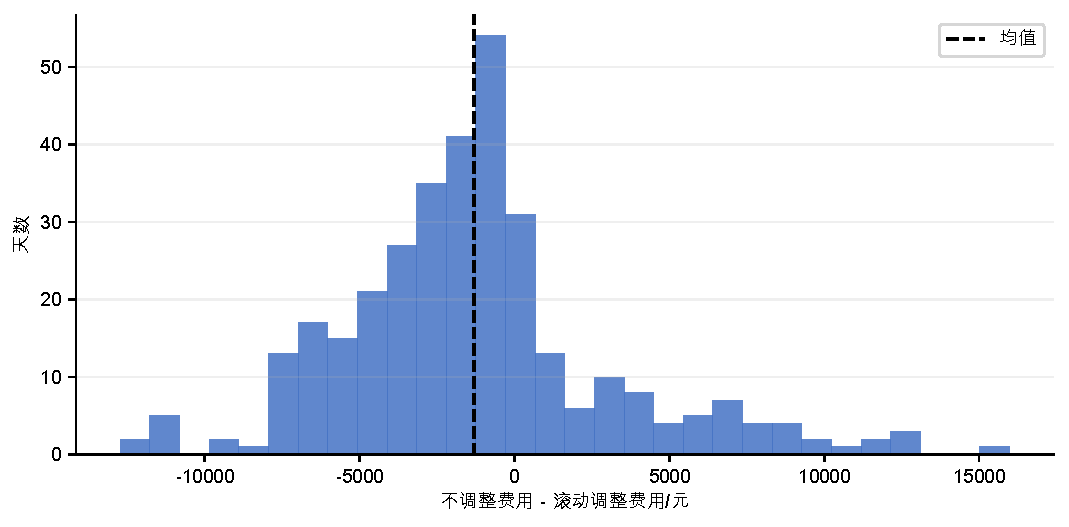
\includegraphics[width=0.90\textwidth]{../figures/fig05_q3_daily_savings.pdf}
\caption{问题三不调整费用与滚动调整费用的逐日差值分布}\label{fig:q3saving}\end{figure}
